\chapter[Introduction]{Chapter 1: Introduction}\label{chap:Proj_Ovv} %Two to three pages long.
%*****************************************************************************************************%
\section{Synopsis}\label{sec:intro1} %Do not give background.
%*****************************************************************************************************%
The research and design in this technical report is focused on advancing energy storage solutions through the development of an innovative Battery Management System (BMS) for Lithium Ferro Phosphate (LFP or LiFePO4) batteries. The initiative seeks to redefine energy storage management paradigms by employing novel methodologies and a distinct architecture, enhancing interactions with comprehensive energy storage mechanisms. This is pivotal for sectors including renewable energy, electric vehicles, bulk energy storage, emergency backup power, and long-term high voltage DC storage.
\begin{quote}
    {\small Battery Management System:\newline
    \emph{a BMS is an electronic system that manages and safeguards a rechargeable battery (cell or battery pack), ensuring optimal performance, prolonged life, and safety. The BMS monitors and regulates various attributes, such as charging and discharging rates, voltage, and temperature. It provides crucial insights and notifications regarding the state of the battery, such as State of Charge (SOC) and State of Health (SOH), while also ensuring the battery operates within safe parameters, thereby protecting against scenarios like overcharging, overheating, or deep discharging which could be detrimental to the battery’s lifespan and performance. In applications like electric vehicles, grid storage, and portable electronics, a BMS plays a pivotal role in ensuring efficient energy utilization, reliability, and safety of the battery usage.}\cite{Trad_BMS}
    }
\end{quote}
\begin{figure}[h!]
\centering
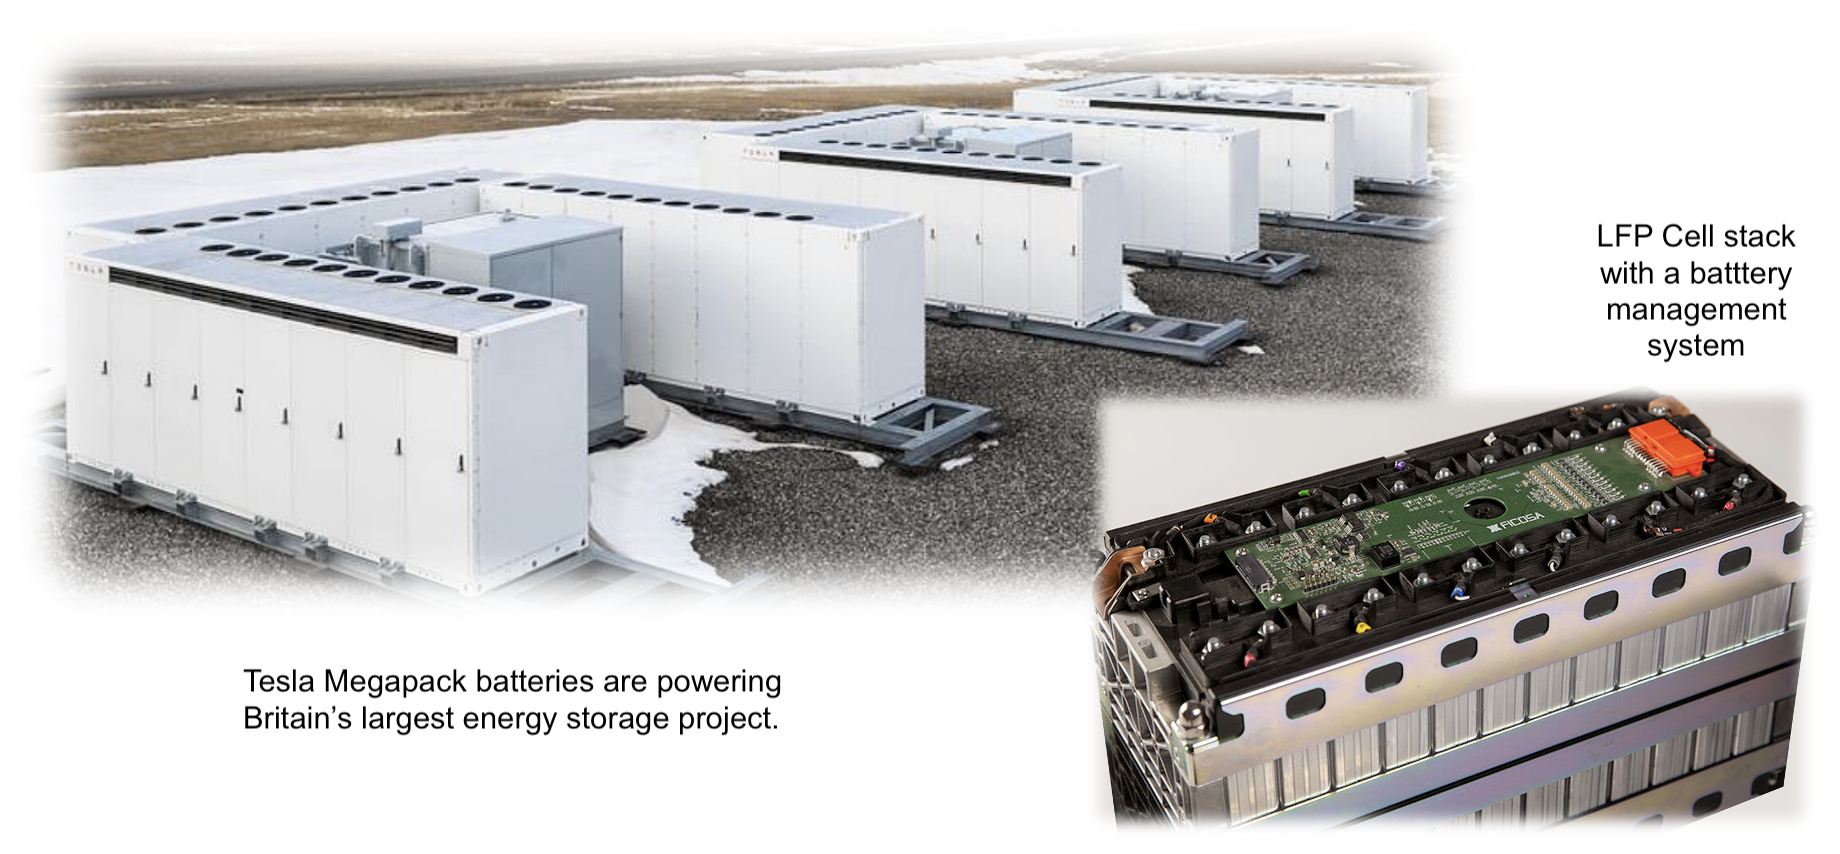
\includegraphics[width=1.0\textwidth]{Skripsie_LaTeXTemplate/Figures/packs.png}
\caption{High Voltage Battery Bank \& a BMS \cite{tessla}}
\label{fig:pak}
\end{figure}
%*****************************************************************************************************%
\section{Problem Statement}\label{sec:probState} %Project motivation: Why do you develop this BMS.
%*****************************************************************************************************%
In the pursuit of developing high voltage battery banks, comprising about 250 cells arranged in series to achieve an approximate voltage of 800V, several significant challenges emerge when interfacing with standard battery management systems (BMS). The primary challenge emanates from the extensive cell strings which, upon connection to a conventional BMS, induce wire overload and inaccurate voltage measurements due to the long wires leading to a single controller, which is ill-suited for precise monitoring across such a vast array of cells.\newline\newline
\noindent
This issue is accentuated by inherent design hurdles associated with high voltage battery banks, such as the imperative need for isolation of communications and transient protection within the BMS to prevent voltage spikes and other transient events, alongside undesirable interactions that could jeopardize system integrity. Accurate state of charge (SOC) and state of health (SOH) estimation of each cell are paramount for safe and efficient battery bank operation.\newline\newline
\noindent
Furthermore, electrical threats like overcurrents, surges, and electrostatic discharge pose additional challenges that the BMS must robustly guard against. The cumulative effect of these challenges elucidates the inadequacy of a single-controller BMS in efficaciously managing and monitoring the numerous cells in high voltage battery banks. Thus, a suitable architecture, that is highly scalable, is desired for the development of high voltage battery banks to overcome the wire overload and inaccurate monitoring predicaments inherent in existing BMS configurations.
%*****************************************************************************************************%
\section{Project Description}\label{sec:projDescrip} %No specific system info or main motivations.
%*****************************************************************************************************%
To address the aforementioned challenges, an innovative design is proposed: deploying a small module with monitoring components and its own micro-controller atop each cell, thereby establishing an individual BMS for each cell. This alternative design significantly mitigates the problem of inaccurate voltage measurements encountered with long wires to a single controller, ensuring a more reliable and robust monitoring system.\newline\newline
\noindent
With voltage measurements taken in close proximity to each cell and facilitated by serial communication between the monitoring modules, a high degree of measurement accuracy is achieved. Initially, the design prototype will be applied to four cells. However, the inherent modular design facilitates seamless scalability, making it adaptable to the high voltage battery bank’s requirements by simply augmenting more cells with modules, fostering a flexible and easily expandable battery management solution.\newpage
\noindent
Although realized through individual module analysis due to logistical and practical constraints, the project's design is fundamentally scalable, allowing for integration into complex, high-voltage systems. The modular BMS, detailed in this report, encompasses hardware design, software development, and performance testing, forming a comprehensive overview of the proposed system.\newline\newline
\noindent
Its modular and adaptable nature guarantees applicability across various domains, positing it as a versatile solution for diverse energy storage requirements, thereby potentially playing a pivotal role in the future energy sector. Through rigorous testing, the superior performance and scalability of the Modular BMS are underscored, demonstrating its potential as a robust and reliable solution for managing Lithium Iron Phosphate (LFP) batteries, and laying a robust foundation for further research and development in battery management technology.
%*****************************************************************************************************%
\section{Report Brief}\label{sec:brief}
%*****************************************************************************************************%
This report presents a detailed review of the project, focusing on the fundamentals of battery management systems and the specifics of the prototype. It covers concepts, design principles, implementation methods, and evaluations, summarizing the project's outcomes and recommendations for future improvements. The flow diagram below provides a structured overview of the report's content.\newline

\begin{figure}[h!]
\centering
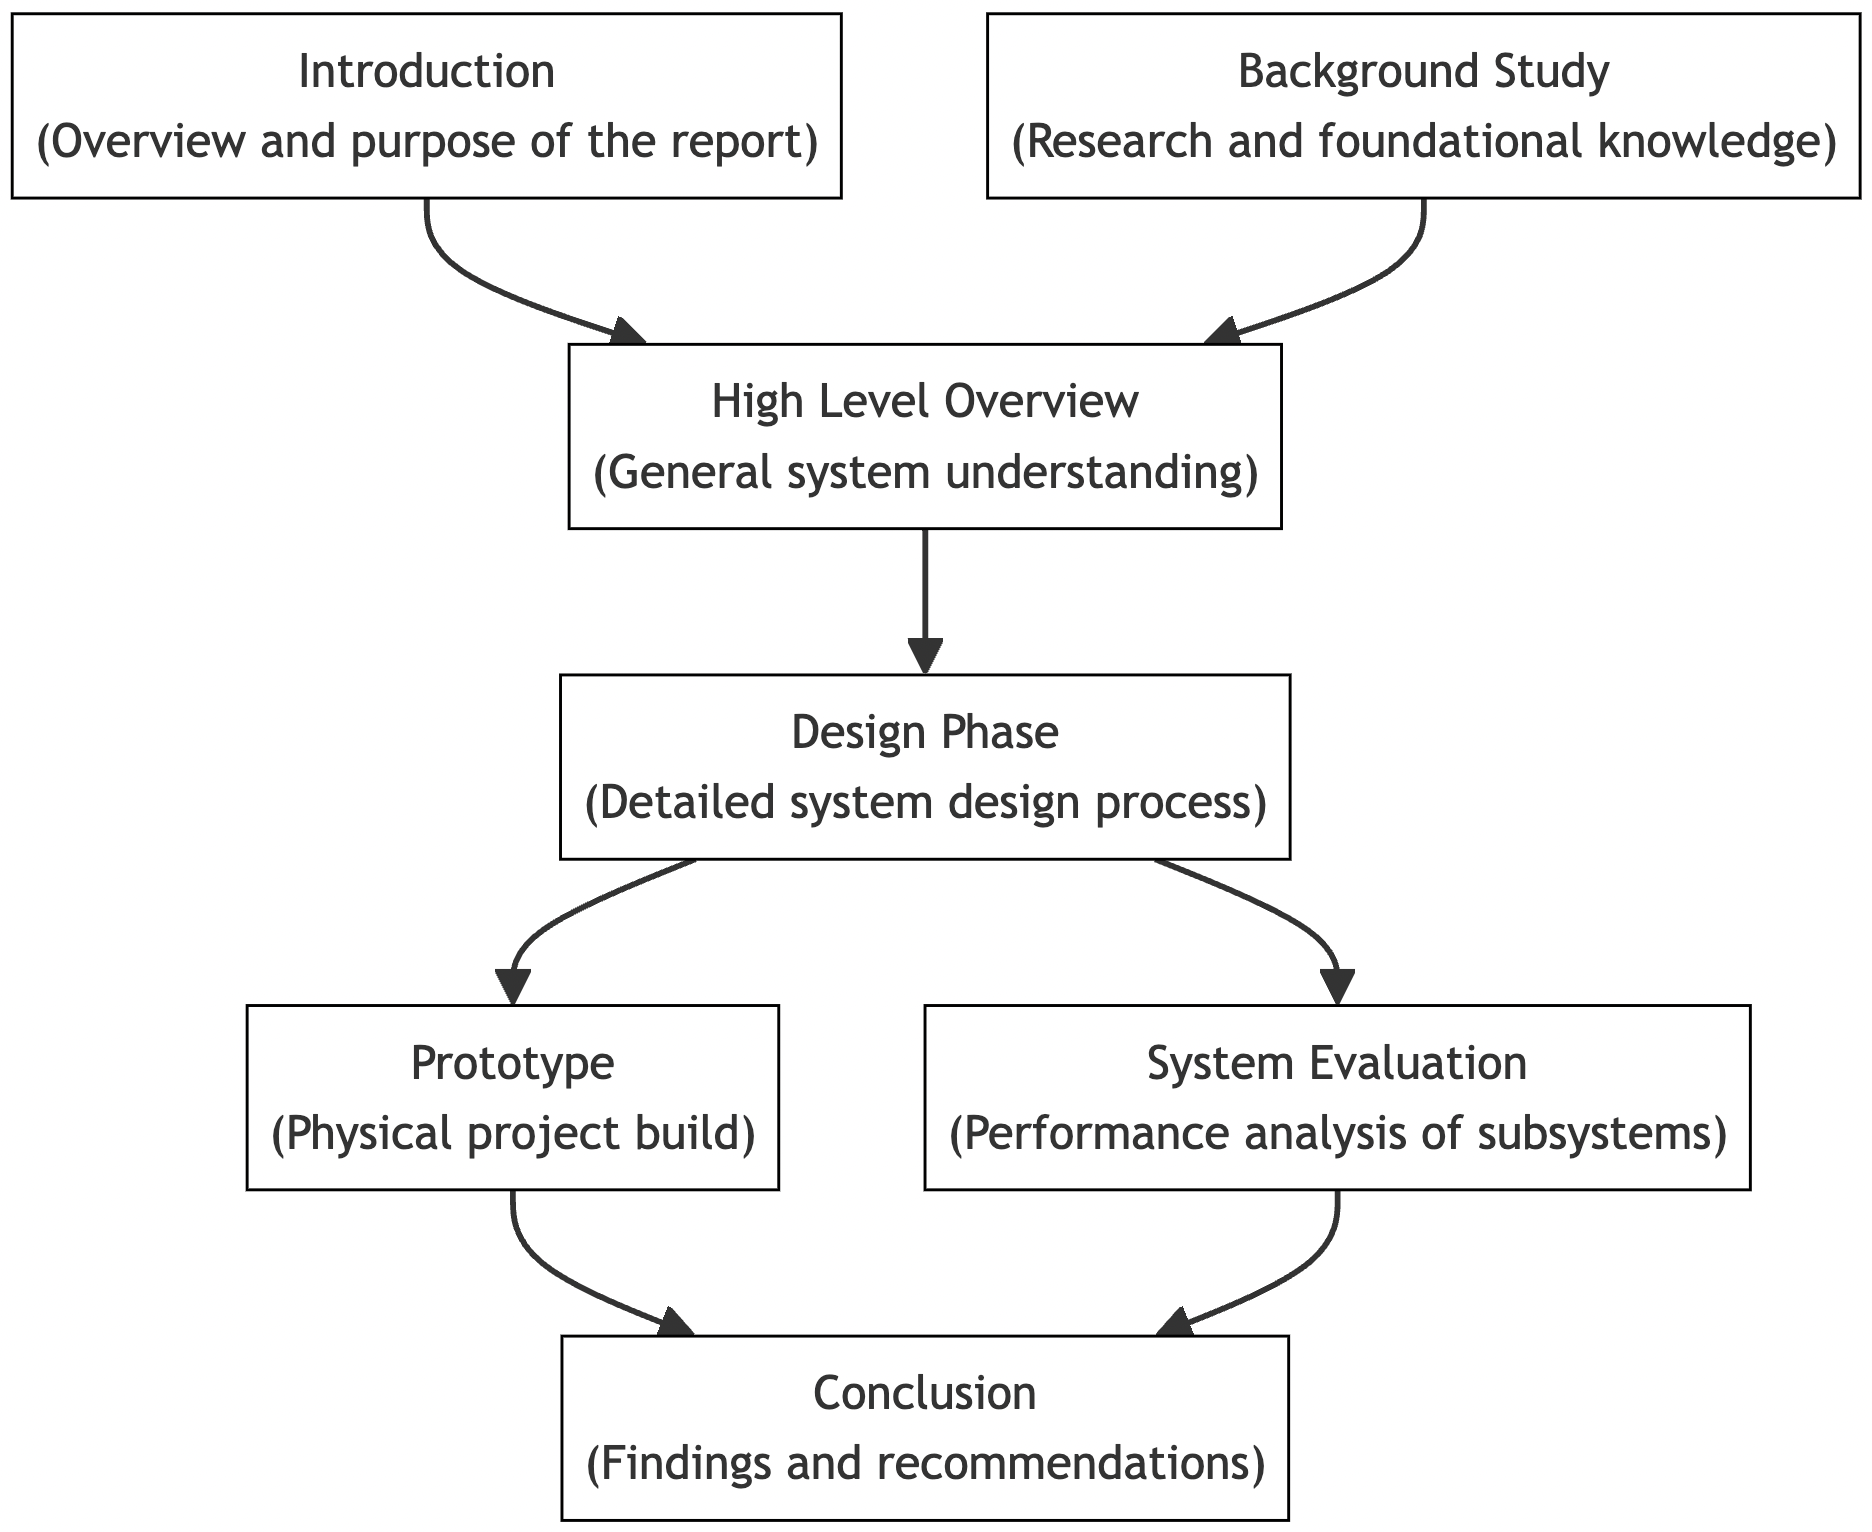
\includegraphics[width=0.7\textwidth]{Skripsie_LaTeXTemplate/Figures/brief.png}
\caption{Report Structured Overview \cite{Mermaid}}
\label{fig:brieff}
\end{figure}

\vfill
